%%%%%%%%%%%%%%%%%%%%%%%%%%%%%%%%%%%%%%%%%%%%%%%%%%%%%%%%%%%
% LaTeX Template ~ 'tau-book.tex'
% Version 2.2 (15/03/2024)
%
% Description: 
% Tau-book is a LaTeX template that offers a clean and 
% professional design for lab reports or academic papers.
% The clarity of the code structure makes it easy to 
% understand and modify for your needs. This template uses 
% an easy-to-read font and high quality equations with "stix2".
%
% Author: 
% Guillermo Jimenez (memo.notess1@gmail.com)
% 
% License:
% Creative Commons CC BY 4.0
%%%%%%%%%%%%%%%%%%%%%%%%%%%%%%%%%%%%%%%%%%%%%%%%%%%%%%%%%%%
%     BIBLIOGRAPHY WITH BIBLATEX IN EXTERNAL EDITORS:
% If the bibliography does not show up, try running the 
% 'tau-book.cls' and 'tau.bib' file with biber from the 
% MikTeX console or your preferred LaTeX distribution to 
% generate the .aux files and (re)run tau-book.tex.
%%%%%%%%%%%%%%%%%%%%%%%%%%%%%%%%%%%%%%%%%%%%%%%%%%%%%%%%%%%

\documentclass[10pt,a4paper,twoside]{tau-book}
\usepackage[italian]{babel}
\usepackage{tau}

%----------------------------------------------------------
% Figure
%----------------------------------------------------------
% Le figure sono quelle prodotte dagli script in Analysis/ e salvate in
% ../figures/: vengono lette direttamente dalla cartella principale del
% progetto, senza mantenerne una copia locale.

\graphicspath{{../}{./}}

%----------------------------------------------------------
% Title
%----------------------------------------------------------

\title{Relazione su un'applicazione del text mining sull'offerta didattica dell'ateneo di Padova}

\author{Cocco Andrea (2040223)} \author{Quartuccio Andrea (2001321)} \author{Varotto Luca (2054021)}
\affil{Corso di Laurea in Statistica per le Tecnologie e le Scienze - Esame di Metodi Statistici per i Big Data}

% Richiesto da tau-book.cls, che usa \@professor nel titolo:
% lasciare vuoto per non stampare alcuna riga.
\professor{}

%----------------------------------------------------------
% Footpage notes
%----------------------------------------------------------

\institution{Università degli studi di Padova}
\ftitle{Relazione su un'applicazione del text mining sull'offerta didattica dell'ateneo di Padova}
\theday{\today}
\course{Esame di Metodi Statistici per i Big Data}

%----------------------------------------------------------

\begin{document}
	
\maketitle

\section{Introduzione}

In questa relazione viene affrontato un problema di Text Mining sull'offerta formativa dell’Università degli Studi di Padova. In particolare si vuole vedere se è possibile classificare gli insegnamenti offerti dai corsi di Laurea triennale dell’ateneo in base alla Scuola di appartenenza. Le otto scuole sono “Scuola di Agraria e Medicina Veterinaria”, “Scuola di Economia e Scienze Politiche”, “Scuola di Giurisprudenza”, “Scuola di Ingegneria”, “Scuola di Medicina e Chirurgia”, “Scuola di Psicologia”, “Scuola di Scienze” e “Scuola di Scienze umane, sociali e del patrimonio culturale”. Nel seguito a quest’ultima ci riferiremo come “Scuola di S.U.S.P.C.”, per brevità espositiva. L'obiettivo è quindi verificare se le descrizioni dei singoli corsi sono molto eterogenee tra di loro e quindi permettono una chiara discriminazione tra le varie Scuole. Altrimenti verranno illustrati i possibili motivi della non eterogeneità tra le descrizioni dei corsi delle Scuole.

\section{La creazione del dataset}

Il dataset è stato creato tramite un programma di web scraping scritto in Python 3.12.3, utilizzando in particolare la libreria BeautifulSoup nella versione 4.12.3. Grazie a questa libreria, è stato possibile esplorare l'intera offerta didattica dell'Università degli Studi di Padova riguardante i corsi di laurea triennali, partendo dal sito https://didattica.unipd.it/off/2021/LT. \\ Per reperire le informazioni necessarie dall'HTML del sito sono stati quindi implementati tre cicli \textit{for} annidati:
\begin{itemize}
    \item il primo per accedere ad ogni Scuola dell'ateneo;
    \item il secondo per accedere ad ogni corso di laurea offerto da ciascuna Scuola;
    \item il terzo per accedere a ciascun insegnamento offerto da ciascun corso di laurea di ciascuna Scuola.
\end{itemize}
Per ogni insegnamento sono stati reperiti due campi di interesse dal Syllabus, ove presenti, ossia “Conoscenze e abilità da acquisire” e “Contenuti”.

In questo modo è stato creato un data-frame che contiene sulle righe ogni insegnamento e sulle colonne sei variabili:
\begin{enumerate}
    \item “School”, corrispondente alla Scuola di appartenenza;
    \item “Degree”, corrispondente al corso di laurea di appartenenza;
    \item “Teaching”,  corrispondente al nome dell'insegnamento;
    \item “Conoscenze”, corrispondente al campo “Conoscenze e abilità da acquisire”;
    \item “Contenuti”,  corrispondente al campo “Contenuti”;
    \item “URL”, corrispondente all'URL del sito.
\end{enumerate}

Nel seguito, per riferirsi a questi campi, si useranno i nomi delle variabili appena introdotte. Il data-frame così creato contiene 3845 righe, che corrispondono ad altrettanti insegnamenti. Grazie alla libreria Pandas, nella versione 2.2.1, questo DataFrame è stato convertito in un file in formato CSV, rendendo così le informazioni facilmente accessibili per le fasi successive.

\section{La pulizia del dataset}

Una volta ottenuto il dataset, la fase di pulizia è stata eseguita in due fasi.

In una prima fase si è affrontato il problema dei dati mancanti. In particolare sono state rimosse le righe in cui sia il campo “Conoscenze” che “Contenuti” erano missing values, ossia NA. In questa categoria rientrano per esempio gli stage, i tirocini o i corsi per ottenere i certificati di lingua.

In una seconda fase si è affrontato il problema dei corsi duplicati. Questo è stato affrontato in tre \textit{steps}:
\begin{enumerate}
    \item Sono state rimosse le righe il cui URL era già apparso in righe precedenti;
    \item Si sono cercati i duplicati nei campi “Contenuti” e “Conoscenze”. Questo è stato fatto grazie alla libreria “digest” per generare hash di testi. Sono state eliminate le righe in presenza di hash duplicati rimuovendo così i “Teaching” duplicati per offerta formativa ma non per URL;
    \item Infine si è affrontato il problema della duplicazione dei “Teaching” per divisione degli studenti (per numero di matricola, iniziali del cognome, o canale). Tra i “Teaching” con le parole “canale”, “pari”, “dispari” o “cognome”, sono stati eliminati quelli con campi “Conoscenze” o “Contenuti” duplicati. Un esempio, può essere rappresentato dal corso “Sperimentazioni di Fisica 1”. Infatti, in questo corso, i professori (diversi per il “Degree” in “Fisica”) si sono suddivisi i studenti in base al cognome (A-L e M-Z). Questo motivo perciò ha portato all'eliminazione del canale “M-Z” del corso citato.
\end{enumerate}

L'ultimo problema riguarda la presenza di alcuni “Teaching” erogati in lingua inglese. Questi hanno quindi i campi “Contenuti” e “Conoscenze” scritti in lingua inglese. Vista la non disponibilità di librerie gratuite online per identificare e tradurre questi testi si è deciso di lasciarli invariati.

Una volta completate tutte le operazioni elencate in precedenza si è arrivati ad avere un dataset con 2092 u.s. Di queste 218 appartenevano alla Scuola di Agraria e Medicina Veterinaria, 192 alla Scuola di Economia e Scienze politiche, 88 alla Scuola di Giurisprudenza, 262 alla Scuola di Ingegneria, 328 alla Scuola di Medicina e Chirurgia, 172 alla Scuola di Psicologia, 447 alla Scuola di S.U.S.P.C. e 385 alla Scuola di Scienze.

\section{Analisi esplorativa aggregata}
\label{sec:analisi_esplorativa_aggregata}

Una volta pulito il dataset si è svolta una prima analisi esplorativa. Prima di farlo, per semplificare le fasi successive, si sono unite le colonne “Contenuti” e “Conoscenze”. La nuova variabile nata dall'unione delle due precedenti è stata chiamata “full.text”. Inoltre, su questa nuova variabile si è deciso di applicare l’analizzatore lessicale “normalizzaTesti” dalla libreria “TextWiller”.
Si è partiti analizzando le tabelle di frequenze, le wordcloud (\textit{Figura} \ref{fig:wordcloud_generale}) e gli istogrammi di frequenza (\textit{Figura} \ref{fig:istogramma_generale}) per le parole nella variabile “full.text”. Da queste si è osservato che le parole più frequenti sono delle parole molto generiche nell'ambito della didattica universitaria, come “corso”, “conoscenze”, “conoscenza” o “studenti”. Ci si aspetta che queste parole non aiutino a discriminare molto tra i vari “Degree” vista la loro generalità.

\begin{figure}[ht!]
    \centering 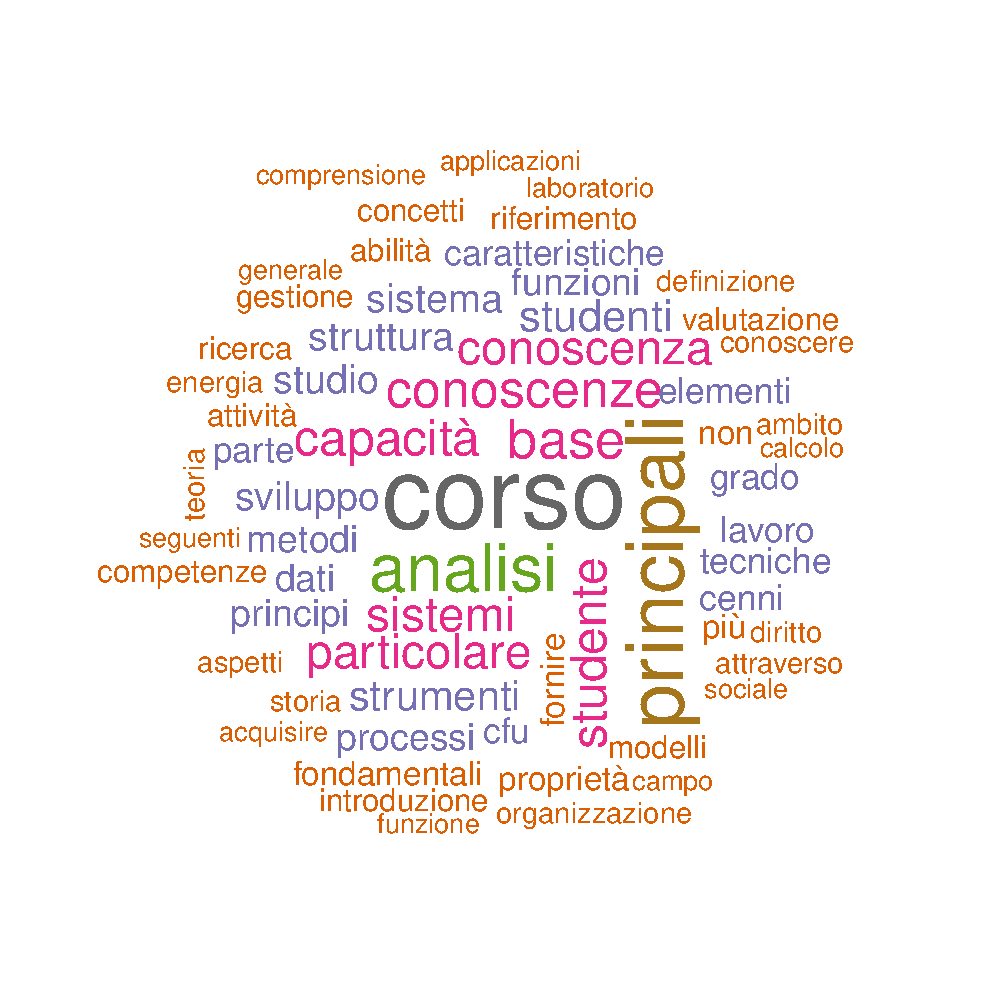
\includegraphics[width=0.48\textwidth]{Figures/wordcloud_generale.pdf}
    \caption{Wordcloud della variabile “full.text” su tutto il dataset.}
    \label{fig:wordcloud_generale}
\end{figure}

\begin{figure}[ht!]
    \centering 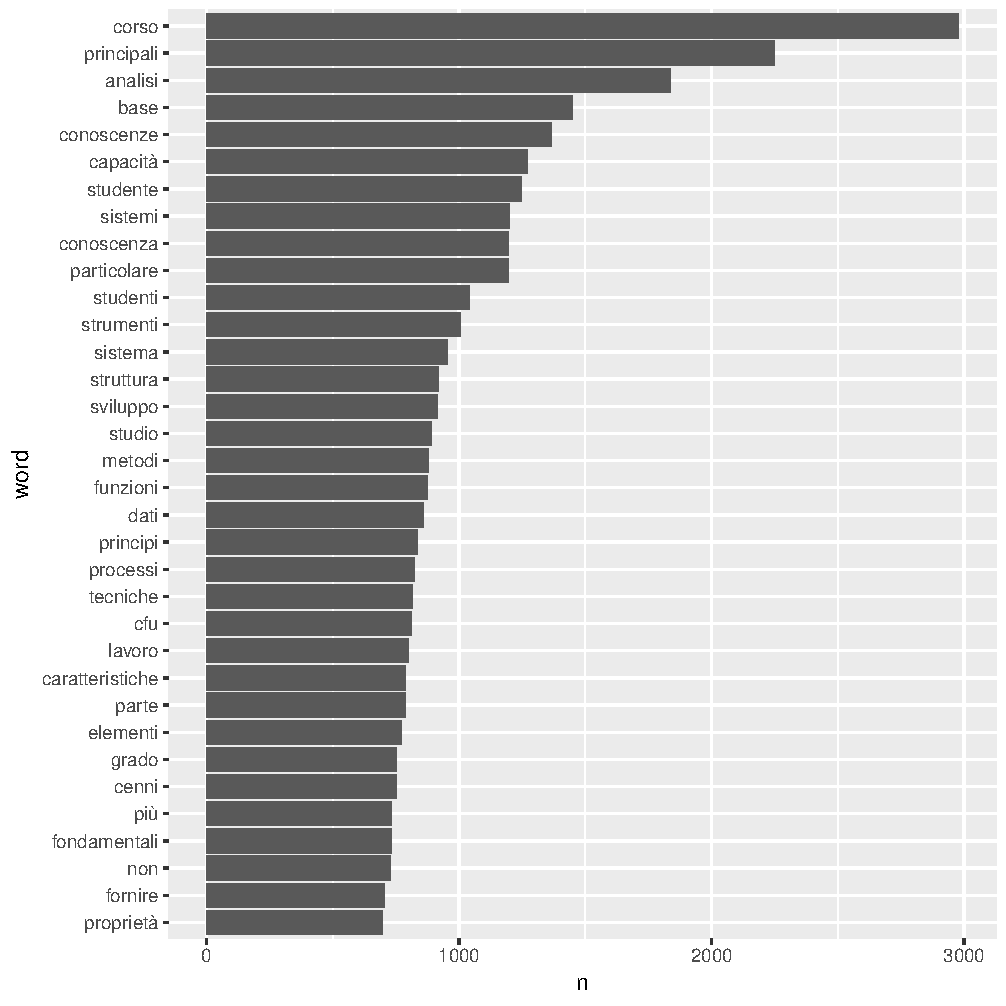
\includegraphics[width=0.48\textwidth]{Figures/istrogramma_generale.pdf}
    \caption{Istogramma della variabile “full.text” su tutto il dataset.}
    \label{fig:istogramma_generale}
\end{figure}

Successivamente si sono cercati i bigrammi e trigrammi più frequenti. Alcuni dei più rilevanti sono: “Unione Europea”, “Corpo Umano”, “Van Der Waals” e “Teorema limite centrale”. Questi concetti sono stati trasformati in un'unica parola sostituendo lo spazio con il carattere ‘\_’.

\subsection{Analisi esplorativa per Scuola}

L'analisi della sezione precedente è stata ripetuta per ogni Scuola e per ognuna sono state trovate molte parole in comune. Allo stesso tempo, sono emerse delle parole tipiche delle singole scuole come “giuridico” e “diritto” per la Scuola di Giurisprudenza (\textit{Figura} \ref{fig:wordcloud_giurisprudenza}) o “storia” e “letteratura” per la Scuola di S.U.S.P.C. (\textit{Figura} \ref{fig:wordcloud_scienze_umane_sociali_patrimonio_culturale}).

\begin{figure}[ht!]
    \centering 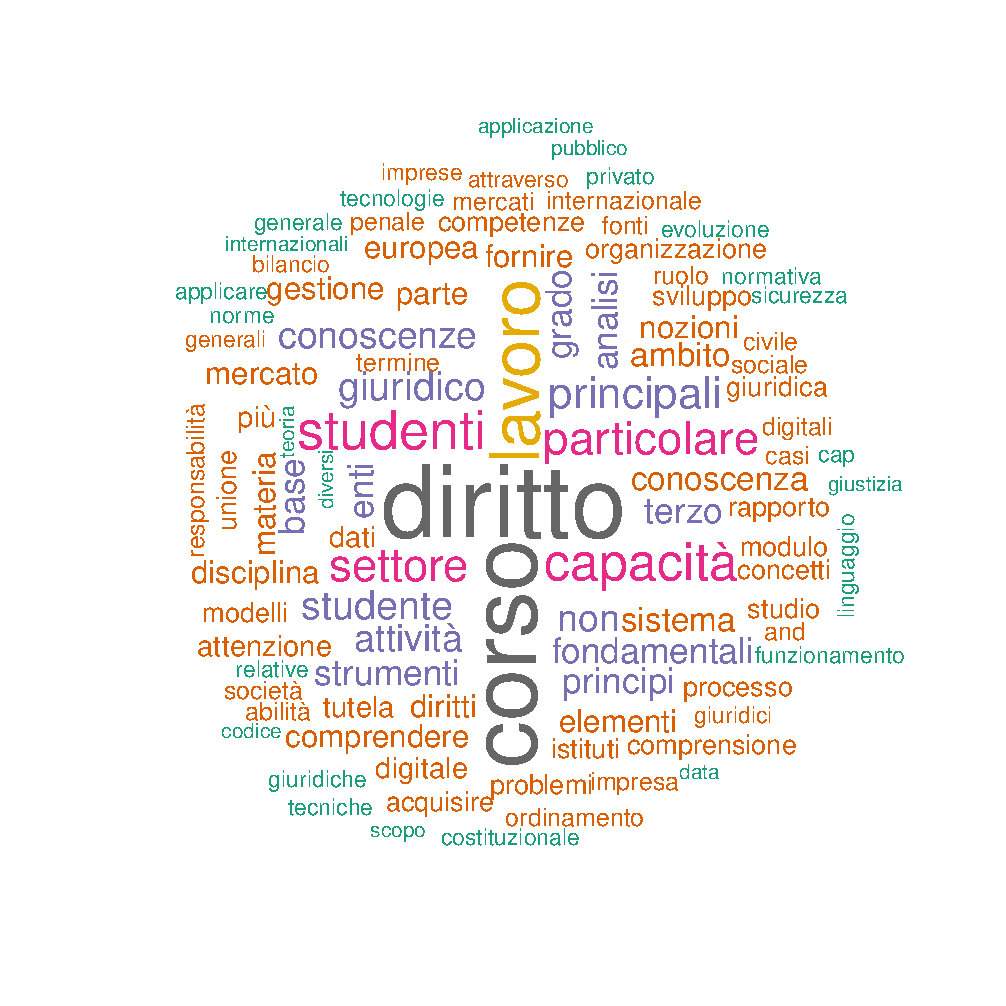
\includegraphics[width=0.48\textwidth]{Figures/wordcloud_giurisprudenza.pdf}
    \caption{Wordcloud della variabile “full.text” sulla Scuola di Giurisprudenza.}
    \label{fig:wordcloud_giurisprudenza}
\end{figure}

\begin{figure}[ht!]
    \centering 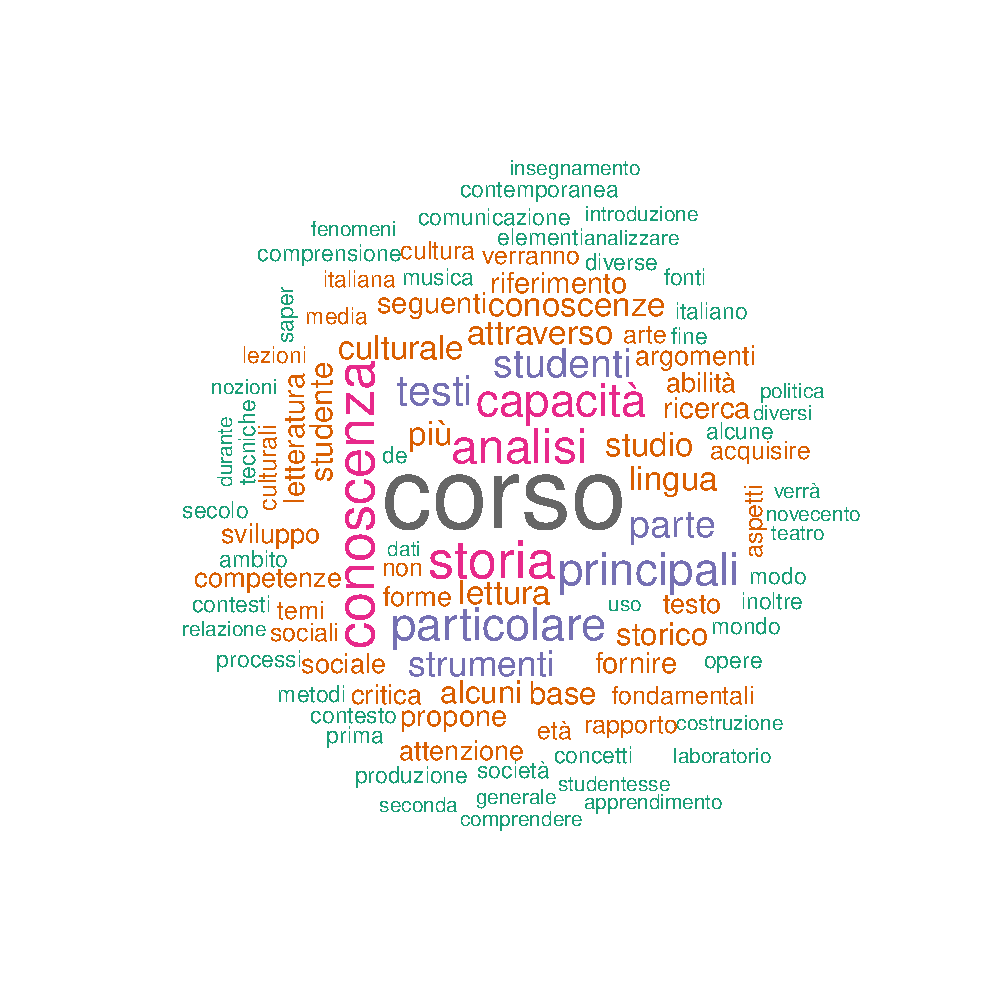
\includegraphics[width=0.48\textwidth]{Figures/wordcloud_ScienzeUmaneSocialiPatrimonioCulturale.pdf}
    \caption{Wordcloud della variabile “full.text” sulla Scuola di S.U.S.P.C.}
    \label{fig:wordcloud_scienze_umane_sociali_patrimonio_culturale}
\end{figure}


\section{Analisi lessicale e stemming}

Visto che nella Sezione \ref{sec:analisi_esplorativa_aggregata} è emersa una grande quantità di parole con la stessa radice si è deciso di eseguire lo stemming del testo. Per farlo è stata usata la funzione “stemDocument” dalla libreria “tm” impostando come lingua l’italiano. 
Dopo questa fase le parole molto frequenti e comuni a tutte le scuole sono state eliminate, in particolare sono stati rimossi gli stem “cors”, “student” e “conoscent”.

\section{Una prima rappresentazione}
\label{sec:una_prima_rappresentazione}

Per proseguire con l’analisi si è determinata la \textit{Document Term Matrix} (DTM) eliminando le parole presenti in meno dello 0.001\% dei documenti.
Si sono quindi calcolatate le componenti principali sui dati standardizzati e il t-SNE bi-dimensionale sulla DTM raggruppata per corso di laurea. Questo raggruppamento dei dati è stato fatto per rendere i grafici successivi più leggibili, visto che in questo modo si è passati dall'avere 2092 u.s. ad averne solo 79. 
I grafici di dispersione sono stati realizzati con l'obiettivo di vedere se i “Degree” appartenenti alla stessa Scuola fossero vicini tra di loro. 
Per la rappresentazione grafica delle PCA si è scelto di usare la seconda e la terza componente poiché erano quelle che fornivano una rappresentazione grafica migliore. Nonostante questo risulta difficile distinguere tutte e 8 le varie scuole.

\begin{figure}[ht!]
    \centering 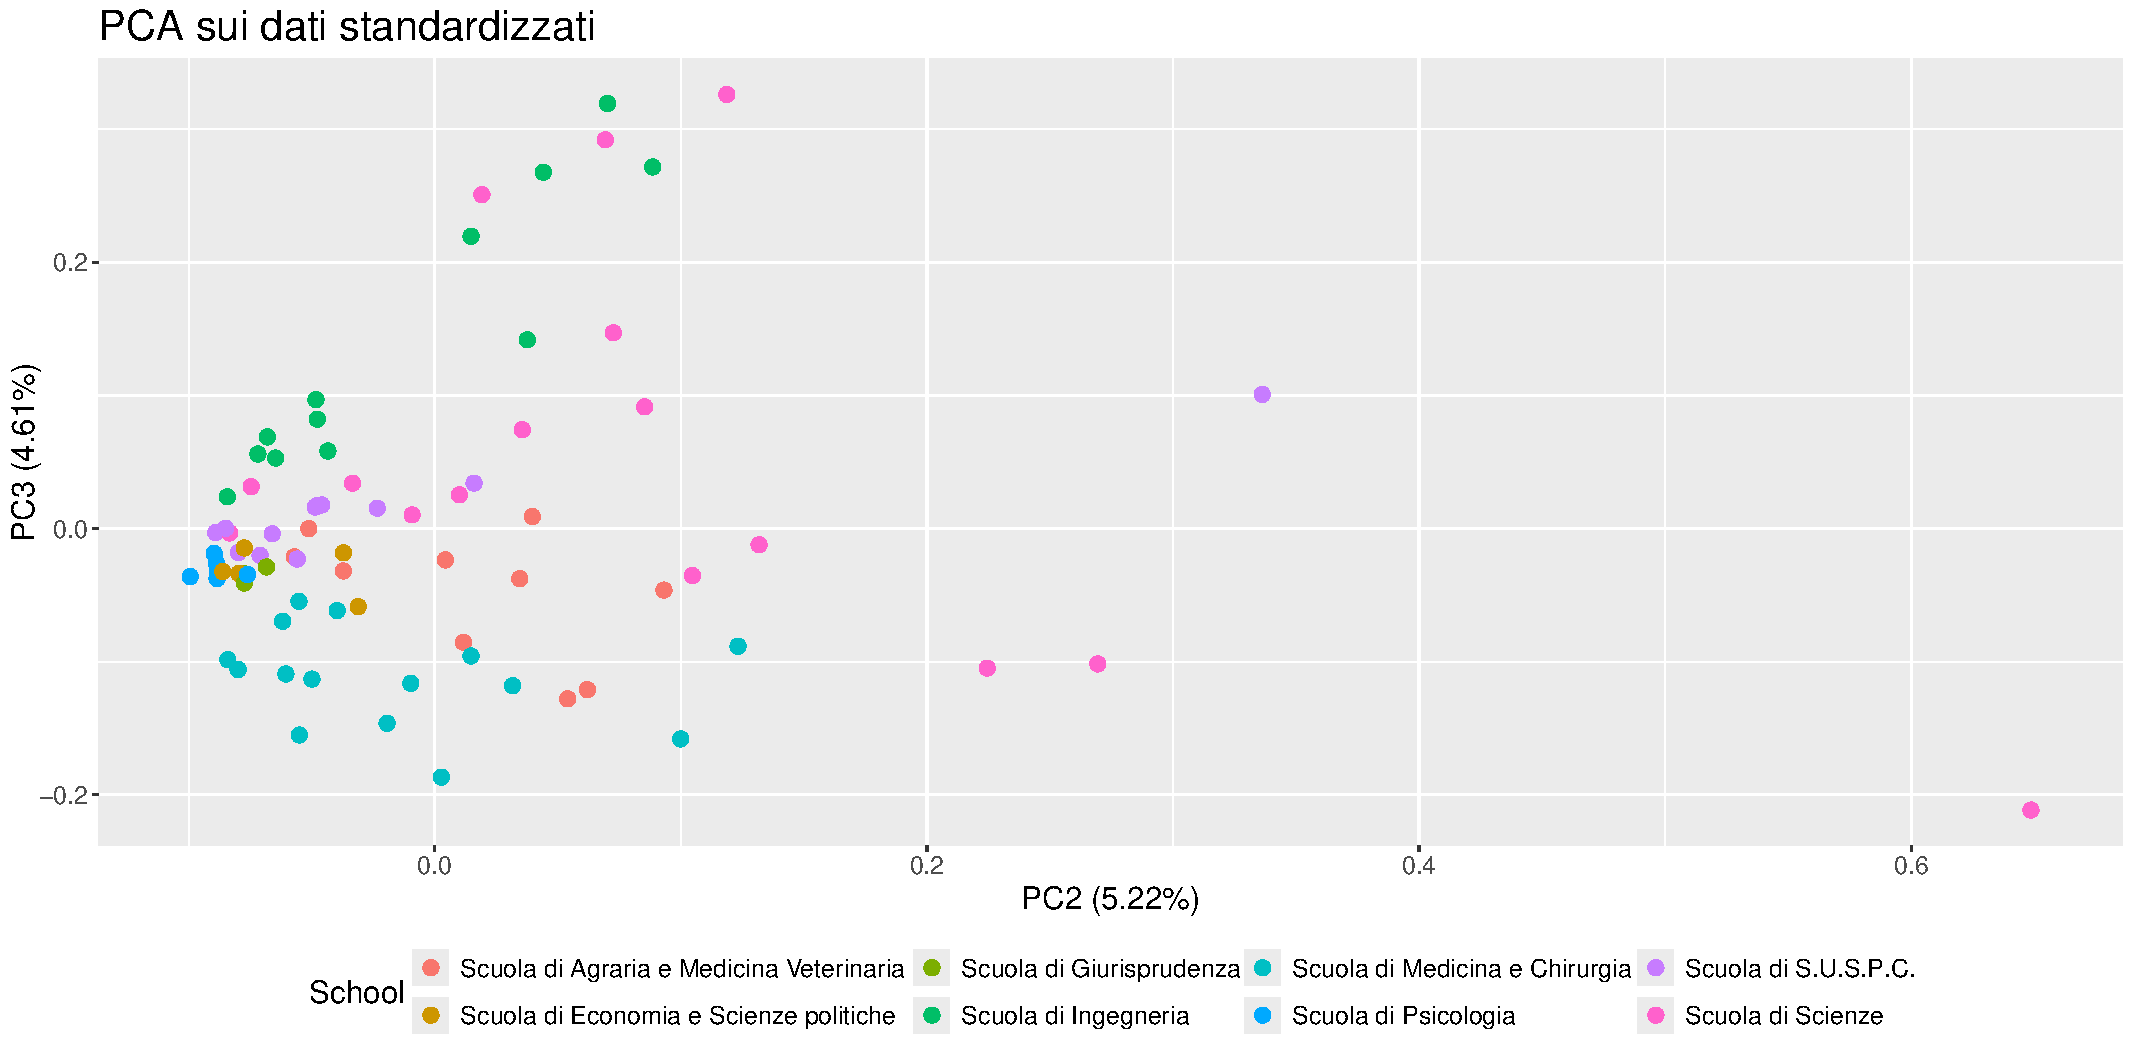
\includegraphics[width=0.48\textwidth]{Figures/pca_s23.pdf}
    \caption{DTM dei “Degree” proiettata sul piano della 2° e della 3° componente principale calcolata sui dati standardizzati.}
    \label{fig:pca_s23}
\end{figure}

\begin{figure}[ht!]
    \centering 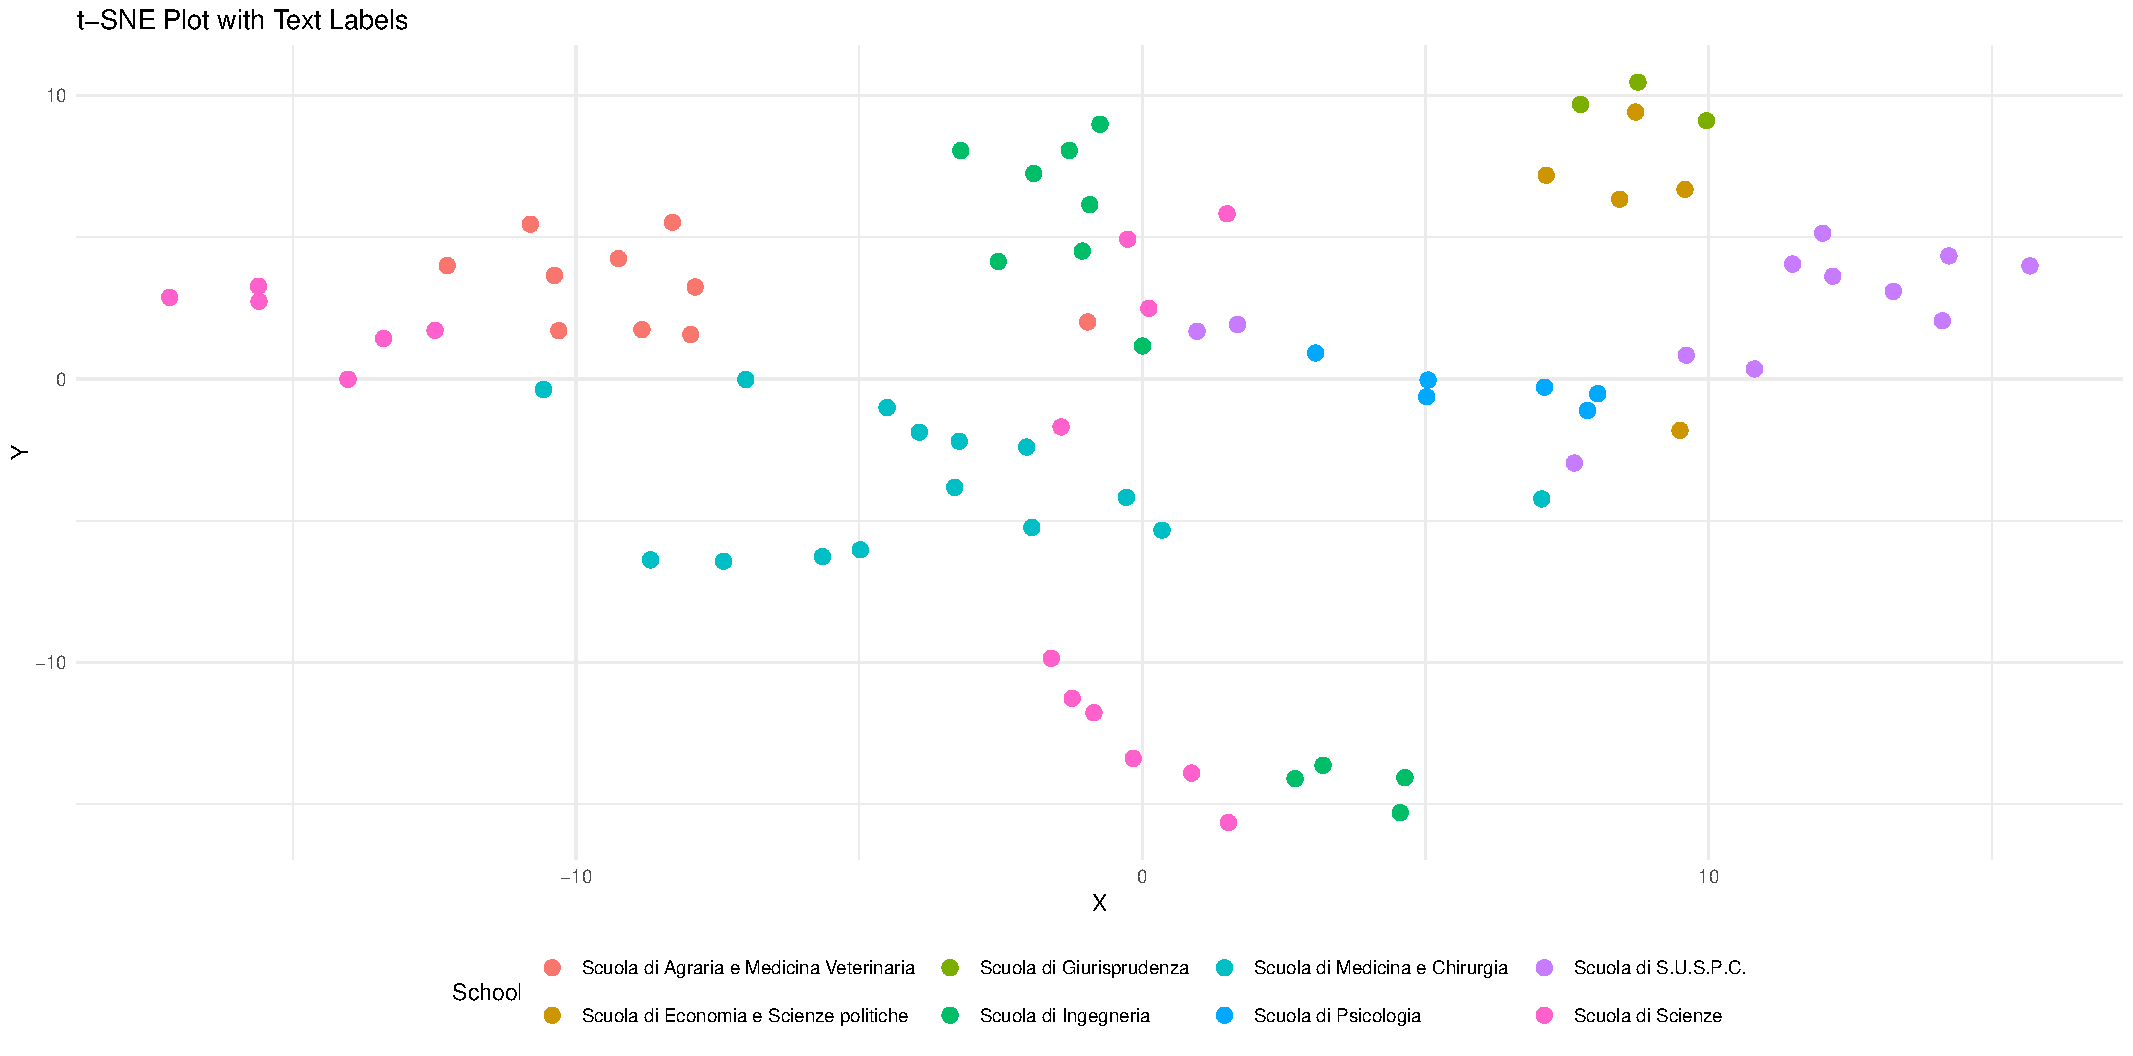
\includegraphics[width=0.48\textwidth]{Figures/t-sne.pdf}
    \caption{Rappresentazione della DTM dei “Degree” tramite t-SNE bidimensionale.}
    \label{fig:t-SNE}
\end{figure}


Dal t-SNE si può distinguere più chiaramente che i “Degree” appartenenti alla stessa Scuola sono vicini tra di loro. Inoltre si nota che i “Degree” che si assomigliano per macro-argomento sono più vicini, come quelli riguardanti le materie scientifiche e le materie umanistiche. Un esempio è che alcuni “Degree” della Scuola di Scienze sono vicini ad alcuni “Degree” della Scuola di Ingegneria, inoltre le osservazioni della Scuola di S.U.S.P.C. sono vicine alla Scuola di Psicologia.

Nel complesso sia la PCA che il t-SNE non ci permettono di riconoscere chiaramente i gruppi relativi ad ogni Scuola. Per questo ci si aspetta una scarsa accuratezza nei modelli di classificazione.

\section{Topic Modelling}
\label{sec:topic_modelling}

Si è provato ad individuare i principali 10 argomenti trattati nel corpus considerando i dati non aggregati; quindi da qui in avanti le u.s. prese in considerazione sono i 2092 “Teaching”. Grazie alla \textit{Latent Dirichlet Allocation} sono stati individuati i seguenti argomenti: Chimica, Medicina, Matematica, Diritto, Biologia, Agraria, Economia, Storia e Letturatura, Fisica e infine Pedagogia. Si è quindi preso un campione di 10 osservazioni casuali e si è determinata la proporzione dei topic più frequenti per ogni osservazione, come si può notare in \textit{Figura} \ref{fig:LDA_sample}. Dal nostro campione inoltre si può vedere che in molti “Teaching” si trattano più argomenti in contemporanea; questo può rappresentare un problema per i modelli di classificazione implementati in seguito.

\begin{figure}[ht!]
    \centering 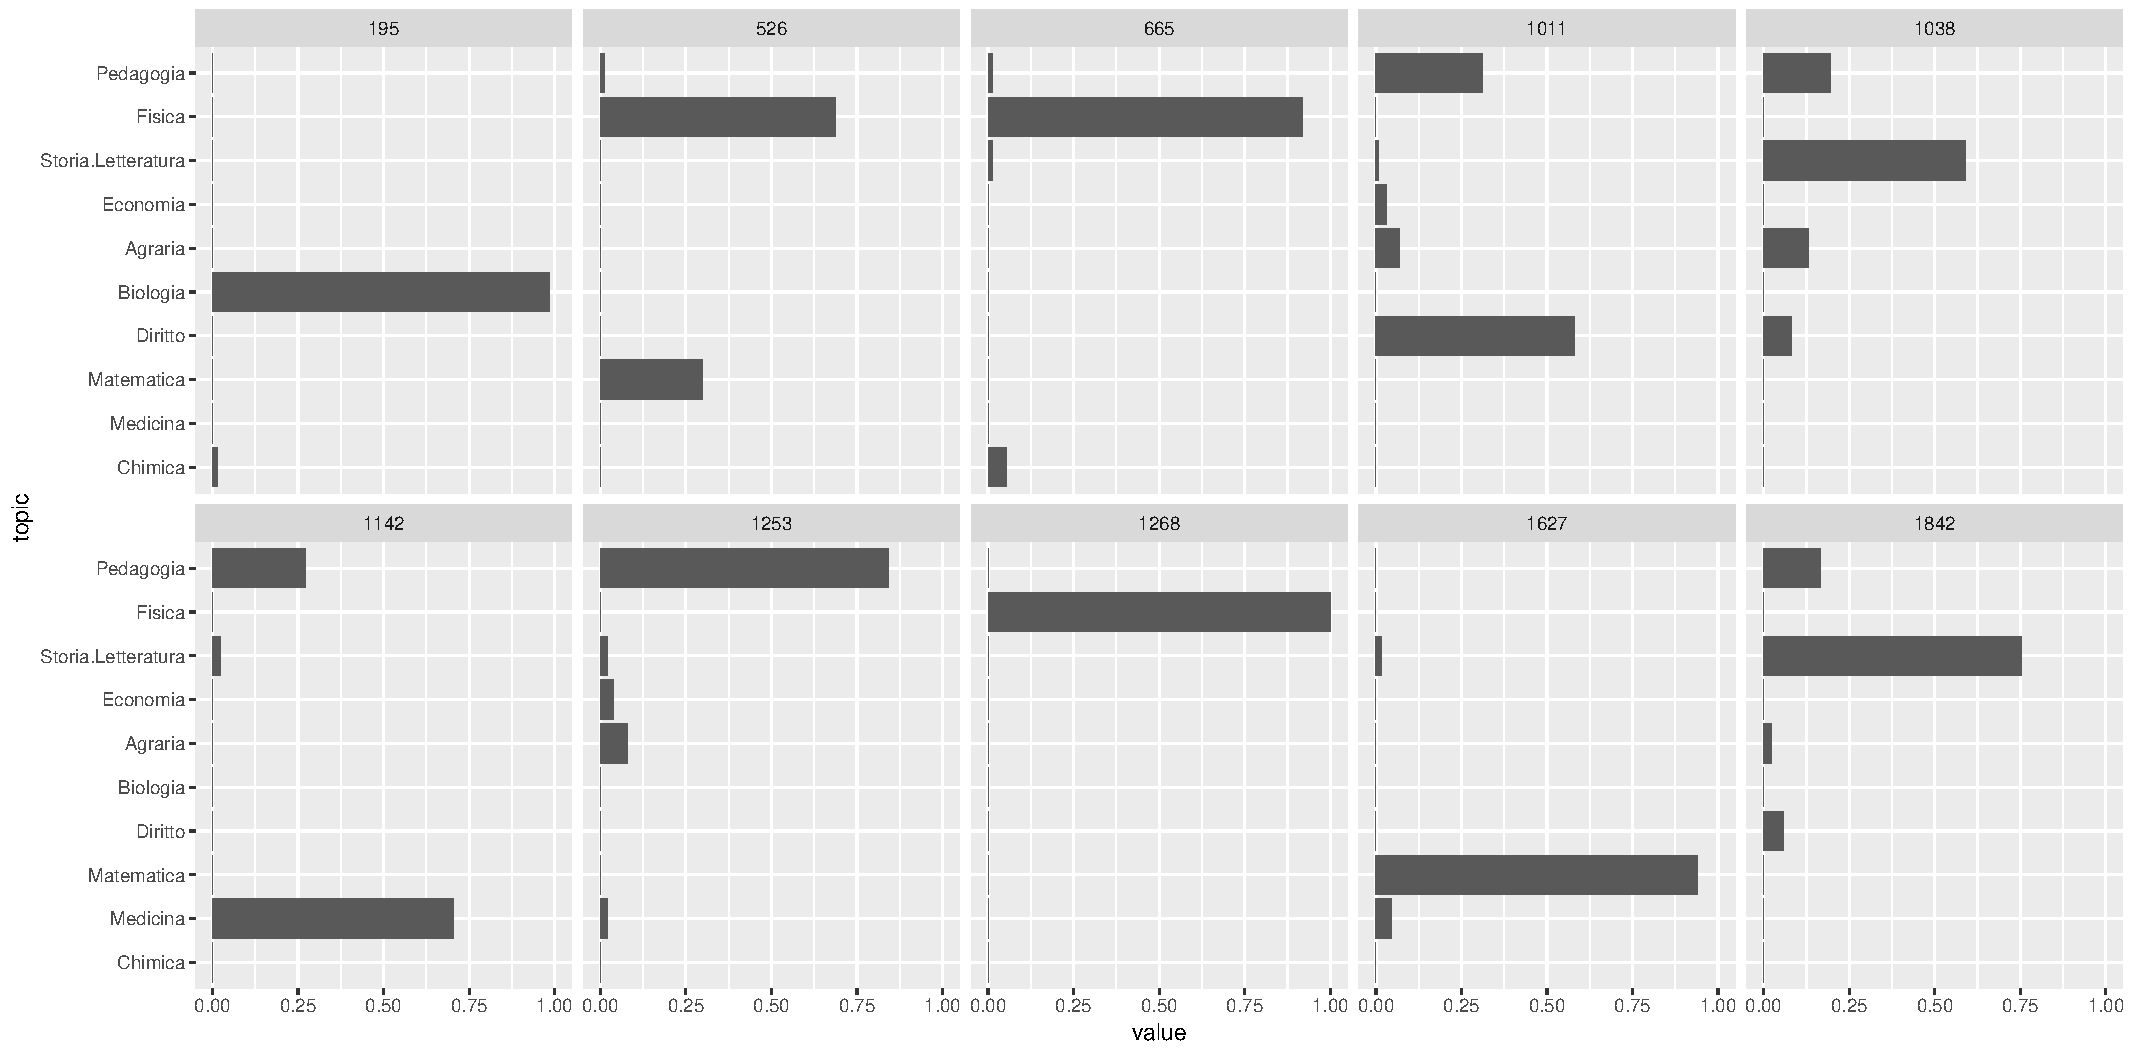
\includegraphics[width=0.48\textwidth]{Figures/lDirichletA_random_sample.pdf}
    \caption{Grafico dei topic più frequenti per un campione di 10 osservazioni casuali.}
    \label{fig:LDA_sample}
\end{figure}
    
\section{I modelli}

In ultima fase è stato valutato l'adattamento dei modelli. Per farlo si è tornati ad utilizzare la DTM avente sulle righe i singoli insegnamenti e la si è divisa in training e test set usando un campionamento stratificato. Questo tipo di campionamento ci permette di mantenere la proporzione dei gruppi nei due campioni. Si tenga presente che la DTM usata ha più colonne che righe ($p>n$), quindi questo ha influenzato la scelta dei modelli.

\subsection{Alberi di Classificazione}
\label{subsec:CART}

Un albero di classificazione è stato adattato quantificando l'impurità con l’indice di Gini. L'albero adattato con questo metodo ha 54 foglie. Da un’analisi dell’errore in cross validation (\textit{Figura} \ref{fig:cv_error_t1}) ci è sembrato opportuno potarlo e ridurlo ad avere 15 foglie, poiché l'errore decresce più lentamente da quel numero di foglie in poi. Potando l’albero l’accuracy cala dal 55\% al 49.2\%, questo però ci permette di rendere l’albero più facilmente interpretabile e riduce il rischio di over-fitting.

\begin{figure}[ht!]
    \centering 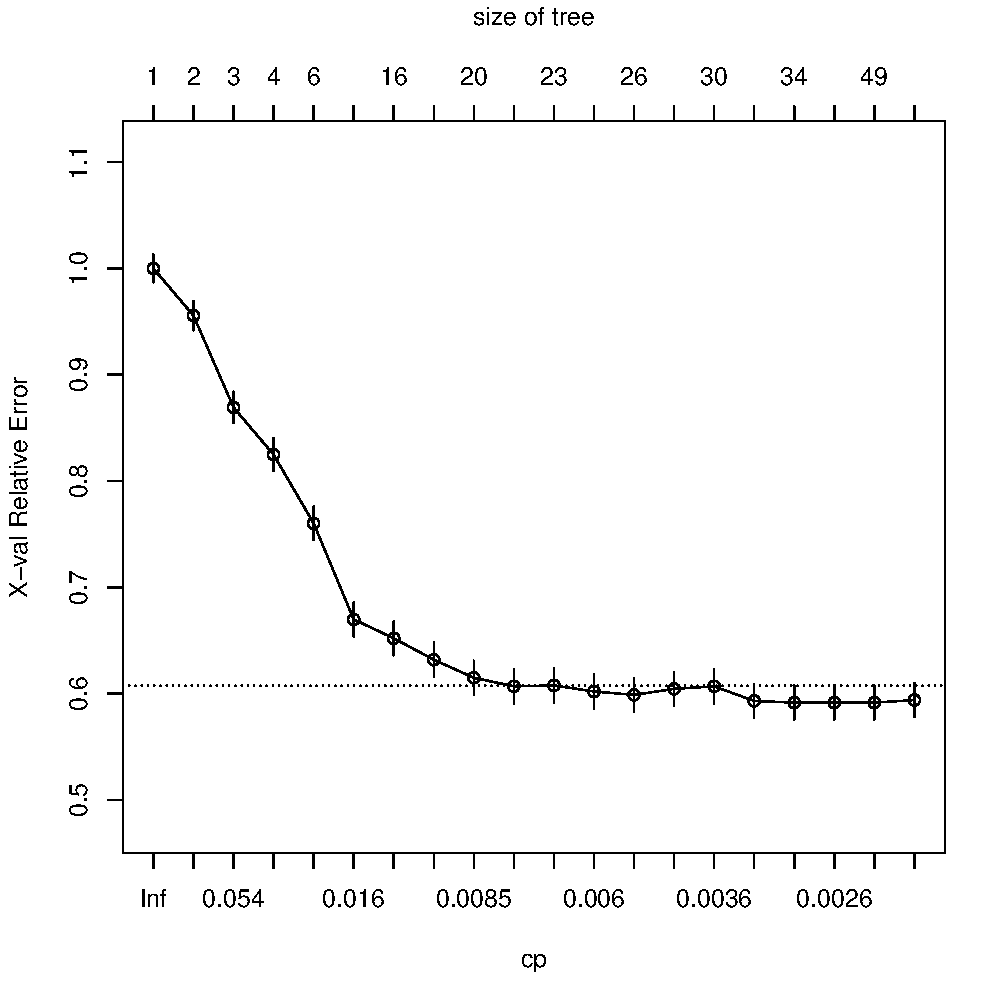
\includegraphics[width=0.48\textwidth]{Figures/cv_error_t1.pdf}
    \caption{Grafico dell'errore in cross-validation dell'albero completo.}
    \label{fig:cv_error_t1}
\end{figure}

L’albero potato è comunque molto grande, ma permette lo stesso di trarre delle conclusioni interessanti. Infatti leggendo gli split nel dettaglio si può vedere per esempio che se la parola “animal” compare almeno una volta l’u.s. viene stimata nella Scuola di Agraria e Medicina veterinaria. Un altro esempio è che se la parola “diritt” compare almeno una volta l’u.s. viene stimata nella Scuola di Giurisprudenza.

Si è provato a vedere nel dettaglio il funzionamento del modello per ogni Scuola. Per esempio si è visto che delle osservazioni relative alla “Scuola di Ingegneria” solo il 21\% viene classificato correttamente, mentre ben il 73\% viene classificato nella “Scuola di Scienze”. Questo errore di classificazione può essere dovuto al fatto che molti corsi tra le due scuole sono in comune, come per esempio i corsi di Analisi Matematica. Un altro esempio è che tra le osservazioni della “Scuola di Agraria e Medicina Veterinaria” solo il 48\% viene classificato correttamente, perché molte osservazioni vengono stimate nella “Scuola di Scienze”. Della “Scuola di Economia e Scienze Politiche” invece solo il 18.75\% delle osservazioni è classificata correttamente, mentre ben il 43\% è stimato nella “Scuola di S.U.S.P.C.”.


\subsection{Neural Network}

Si è stimata una rete neurale con un layer ed otto nodi. Nello stimarla ci si è basati sulla DTM che tiene le parole che appaiono in almeno il 2.5\% dei documenti, questo ha portato a ridurre il numero di colonne della matrice ma è stato fondamentale per ridurre i tempi computazionali della stima e per raggiungere convergenza. Tale modello ha raggiunto convergenza dopo 710 iterazioni e il modello applicato sul training set ha una accuracy del 67\%. Questo modello è molto più preciso di quello con gli alberi ma ci fa perdere completamente l’aspetto interpretativo.

Si è provato a vedere nel dettaglio il funzionamento del modello per ogni Scuola. Per esempio si è visto che delle osservazioni relative alla “Scuola di Ingegneria” il 73\% delle u.s. viene classificato correttamente, mentre il 12\% viene classificato nella “Scuola di Scienze”. Mentre delle osservazioni relative alla “Scuola di Scienze” ne vengono correttamente classificate solo il 51\%, invece il 15\% vengono messe nella “Scuola di Ingegneria”.

\section{Un altro schema di pesatura}

Infine i vari modelli sono stati riadattati cambiando lo schema di pesatura nel calcolo della DTM. In particolare si è passati dal \textit{TF} (\textit{Term Frequency}), usato in precedenza, al \textit{normalizaed TF-IDF} (\textit{Term Frequency-Inverse Document Frequency}). In particolare dato il documento j-esimo e la parola i-esima i due si calcolano nel seguente modo:
\begin{equation}
\begin{aligned}
    TF_{i,j}\text{: }&n_{i,j} \\ \text{Normalized }TF-IDF_{i,j}\text{: }& \left( \dfrac{n_{i,j}}{\sum_k n_{k,j}} \right) \cdot \log_2 \left( \dfrac{N}{|d:i\in d|} \right)
\end{aligned}
\end{equation}
dove $n_{i,j}$ indica le occorrenze dalla parola i nel j-esimo documento, N indica il numero totale di documenti nel corpus e d indica il generico documento nel corpus.
L'albero di classificazione potato ha una precisione del 54\% sul test set, nonostante abbia due foglie in meno. La nuova Rete Neurale invece raggiunge la convergenza dopo 850 iterazioni ed ha una precisione del 68\%. Si può quindi dire che questo schema di pesatura migliori leggermente i risultati; non è possibile sapere se questo incremento sia significativo o meno, potrebbe essere dovuto ad un particolare split di training e test set o ad altri fattori esterni. Un altro aspetto da considerare di questo schema di campionamento è la perdita di interpretabilità. Infatti è molto più intuitivo classificare le osservazioni in base alla loro frequenza che in base al loro \textit{normalized TF-IDF}. Per esempio nella sezione \ref{subsec:CART}, dove è stato usato il TF, si è visto che se la parola “diritt” appare almeno una volta nel testo l'u.s. verrà classificata nella “Scuola di Giurisprudenza”. Tale discorso non può essere fatto con il TF-IDF perché bisogna considerare anche la lunghezza del singolo testo e la frequenza della parola nei documenti del corpus.

\section{Conclusioni}

In conclusione la precisione dei modelli stimati, a prescindere dallo schema di pesatura, non è altissima. La Neural Network, essendo uno strumento più flessibile, ha una maggiore precisione in questa particolare applicazione. Nonostante la maggiore precisione fa comunque fatica a classificare correttamente alcune Scuole. Gli alberi, invece, hanno maggiore interpretabilità ma funzionano peggio per discriminare alcune Scuole come quella di Ingegneria e di Scienze.
Questo ci fa capire che i due campi selezionati dal Syllabus, cioè “Conoscenze e abilità da acquisire” e “Contenuti” non bastino a discriminare perfettamente tra le varie Scuole. Questo problema può essere dovuto al fatto che Scuole diverse, come quella di Scienze ed Ingegneria, trattino argomenti simili e quindi abbiano molte parole in comune nelle descrizioni dei loro corsi. Per esempio in queste due Scuole sono ricorrenti gli esami in cui si parla di Matematica e di Fisica. Questa sovrapposizione la si può vedere dalle rappresentazioni grafiche della \textit{Sezione} \ref{sec:una_prima_rappresentazione} e dal Topic Modelling effettuato nella \textit{Sezione} \ref{sec:topic_modelling}.

\section{Bibliografia}

$[1]$ Hastie, Tibshirani, Friedman (2009). \textit{The elements of statistical learning}. Springer, Berlin. \\ $[2]$ \textit{Slides del corso di Metodi Statistici per i Big Data},  A. Canale, F. Denti, B. Scarpa. \\ $[3]$ \textit{Information Retrieval, macchine e motori di ricerca},  M. Melucci.

\end{document}